\documentclass[manuscript,screen,review]{acmart}

\AtBeginDocument{%
  \providecommand\BibTeX{{Bib\TeX}}}

\title{DaCc: Difficulty-adaptive and Caption-consistent Notes-guided MLLM Reasoning for KB-VQA}

\author{Jian Li}
\affiliation{
  \institution{School of Computer Science and Engineering, Macau University of Science and Technology}
  \city{Macau}
  \country{China}}
\email{3250001785@student.must.edu.mo}
\orcid{0009-0001-1701-7496}

\renewcommand{\shortauthors}{Li et al.}

\begin{document}

\begin{abstract}
Knowledge-based Visual Question Answering (KB-VQA) requires the effective integration of external information from vast knowledge bases to answer questions that go beyond the visual content of an image. Current methods often struggle with fixed retrieval counts and imprecise knowledge refinement, leading to the inclusion of irrelevant noise or insufficient context for complex queries. In this paper, we propose a novel framework featuring an adaptive top-k retrieval strategy and a bidirectional refinement mechanism. Our approach dynamically determines the optimal number of knowledge passages based on question difficulty and utilizes deep multimodal semantic similarity to refine knowledge notes. This ensures high correspondence between visual features and retrieved text. By filtering irrelevant information and enhancing semantic alignment, our method significantly improves the quality of knowledge integration. Experimental results on mainstream benchmarks demonstrate the effectiveness of our approach, which chieves competitive performance on both the OK-VQA and A-OKVQA datasets, closely approaching the state-of-the-art methods.
\end{abstract}

\keywords{knowledge-based visual question answering, adaptive retrieval, multimodal reasoning, knowledge refinement}

\maketitle

\section{Introduction}

Visual Question Answering (VQA) has progressed from recognition-centric benchmarks toward open-ended reasoning settings in which the answer cannot be inferred from pixels alone. In these scenarios, a model must interpret objects, attributes, spatial cues, and latent intent in the question, and then connect them with background facts such as commonsense knowledge, encyclopedic information, or domain-specific descriptions. Knowledge-based VQA (KB-VQA) therefore sits at the intersection of visual grounding, information retrieval, and language reasoning, making it one of the most challenging tasks in multimodal intelligence.

Recent Multimodal Large Language Models (MLLMs) have substantially improved zero-shot and few-shot VQA performance by leveraging large-scale pretraining and strong instruction-following ability. Nevertheless, their internal knowledge is often incomplete, outdated, or weakly aligned with the current image. When a question asks why a tool is used, which event a monument commemorates, or what biological function an observed object serves, pure parametric reasoning is frequently insufficient. In such cases, the model benefits from access to external evidence, but only if that evidence is relevant, compact, and synchronized with the visual scene.

A major limitation of existing KB-VQA pipelines is that retrieval is commonly treated as a fixed preprocessing step. Most systems fetch a constant number of passages for every sample, regardless of whether the question is simple and localized or compositional and evidence-intensive. This design introduces a persistent trade-off. When too few passages are retrieved, the model lacks the factual coverage needed for multi-hop reasoning; when too many passages are retrieved, irrelevant text overwhelms the context window and increases the chance of hallucinated answers. The problem becomes more severe when retrieved passages are only loosely related to the objects or regions that actually determine the answer.

Another challenge lies in the semantic mismatch between text retrieval and visual grounding. Retrieved evidence may be topically related to the question, yet still fail to match the image instance under consideration. For example, a passage about the general function of a device may be useful only if the model can first verify that the device is indeed present and salient in the image. Similarly, OCR tokens and generated captions may expand the retrieval space, but they also introduce lexical noise and distract the model from the truly discriminative visual content.

To address these issues, we propose an adaptive and alignment-aware KB-VQA framework. The first component is an adaptive top-$k$ retriever that predicts how much external evidence is needed for each question. Instead of committing to a single retrieval budget, the model analyzes query difficulty and the distribution of retrieval scores to decide whether a narrow or broad evidence pool is more appropriate. The second component is a bidirectional refinement module that improves both modalities: textual knowledge is compressed into concise knowledge notes, while image features are filtered into visual notes conditioned on the refined text. This two-way interaction reduces irrelevant context and promotes semantically grounded reasoning.

Our method is designed around a simple intuition: for KB-VQA, better answers do not merely require more knowledge, but better coordinated knowledge. By explicitly controlling retrieval breadth and by iteratively aligning retrieved text with image evidence, the framework creates cleaner inputs for the final reasoning stage. This design improves robustness to noisy passages, supports multi-step reasoning, and yields a more interpretable reasoning pipeline through intermediate notes.

The main contributions of this paper are threefold. First, we introduce an adaptive top-$k$ retrieval strategy that dynamically adjusts the amount of external evidence to the difficulty of each query. Second, we design a bidirectional refinement mechanism that distills retrieved passages into knowledge notes and grounds them through question-aware visual note generation. Third, we show that the resulting framework offers a practical way to improve KB-VQA performance while reducing the burden of redundant context in downstream MLLM reasoning.

\section{Related Work}

\subsection{Knowledge-based VQA}

Early KB-VQA methods relied on structured resources such as DBpedia, ConceptNet, or handcrafted knowledge graphs, where question answering was formulated as entity linking followed by symbolic reasoning. These approaches provided explicit supervision paths, but they were often brittle in the presence of visual ambiguity and linguistic variation. As multimodal pretraining matured, the field gradually shifted toward unstructured evidence retrieval from large corpora such as Wikipedia, web documents, and caption repositories. This transition made it easier to cover long-tail concepts, but it also made evidence selection substantially noisier.

A representative direction in recent KB-VQA research is to augment the question with image-derived text, including OCR tokens, dense captions, object tags, or scene summaries, and then use the resulting query for dense retrieval. Systems such as TRiG and related retrieval-augmented models demonstrate that visually enriched queries can improve recall over relevant passages. More recent methods further integrate MLLMs as answer generators on top of retrieved evidence, allowing the model to reason over image content and external text in a unified prompting framework. However, many of these systems still inherit a static retrieve-then-read design, where the number and structure of retrieved passages remain unchanged across samples.

The framework most related to our work is the notes-guided line of KB-VQA research, exemplified by approaches that transform raw passages into compact textual notes and combine them with visual cues during reasoning. This family of methods shows that compressed evidence is often more useful than raw passages because it reduces context length and suppresses distractors. Our work builds on this insight but argues that note generation alone is not enough: the retrieval budget should also be adaptive, and the refinement stage should explicitly operate in both textual and visual directions.

\subsection{Retrieval-Augmented Generation for Multimodal Reasoning}

Retrieval-Augmented Generation (RAG) has become a standard paradigm for extending large language models with non-parametric memory. In the unimodal setting, RAG improves factuality and adaptability by retrieving supporting documents at inference time and conditioning generation on them. In multimodal tasks, this idea has been extended to image-grounded dialogue, multimodal chain-of-thought prompting, and VQA with external evidence. Methods such as KAT, REVIVE, and other knowledge-enhanced MLLM pipelines show that retrieved text can meaningfully improve answer accuracy when the question cannot be solved from the image alone.

Despite these advances, multimodal RAG methods often underutilize the interaction between retrieval and reasoning. Retrieval is typically executed once using a query composed of the question and coarse image descriptors, after which the downstream generator passively consumes all returned passages. This one-shot design overlooks two important facts. First, uncertainty is not uniform across questions; therefore, a fixed top-$k$ budget is rarely optimal. Second, the utility of a passage depends on whether it can be aligned with the specific visual evidence in the current sample. A passage that is semantically related in a global sense may still be unhelpful if it does not correspond to the relevant object, action, or region in the image.

Our approach can be viewed as a query-aware and visually grounded extension of multimodal RAG. Rather than treating retrieval as an immutable front-end, we let the retrieval budget respond to question complexity and use refinement to feed information back into the multimodal representation space. This design preserves the strengths of retrieval-augmented reasoning while reducing the mismatch between retrieved evidence and answer-critical visual content.

\subsection{Multimodal Semantic Alignment}

A parallel line of work focuses on aligning visual and textual representations so that information can be transferred more reliably across modalities. Contrastive pretraining methods such as CLIP established a strong foundation for image-text matching at global scale, while subsequent models explored fine-grained alignment between words, regions, patches, and object proposals. In VQA and referring expression tasks, these techniques improve grounding by encouraging the model to attend to the portions of the image that best correspond to the linguistic input.

For KB-VQA, alignment plays a slightly different but equally important role. The core difficulty is not only matching a question to an image, but also matching retrieved knowledge to the right evidence in the image. If the model cannot determine which retrieved facts are visually instantiated, reasoning quality degrades even when retrieval recall is high. Several recent works attempt to address this issue by using cross-attention, region-level relevance scoring, or MLLM-based summarization to filter either the text or the image. However, most methods prioritize one direction of refinement and leave the other modality largely untouched.

We argue that effective KB-VQA requires bidirectional alignment. Textual evidence should be condensed into short, answer-relevant notes, and visual evidence should be re-expressed through regions or summaries that are conditioned on those notes. By alternating these two operations, the model narrows the semantic gap between the retrieved corpus and the specific scene under analysis. This idea motivates the design of our method section.

\section{Methodology}

\subsection{Overview}

The overall framework of our proposed method is illustrated in Fig.~\ref{fig:framework}. Given an input image $V$, a question $q$, and an external knowledge base $\mathcal{K}$, our goal is to retrieve useful external knowledge from $\mathcal{K}$ and provide reliable answers to $q$ based on image $V$. Existing notes-guided reasoning methods usually retrieve a fixed number of top-$k$ knowledge passages from the knowledge base and then summarize them into knowledge notes for subsequent reasoning. However, such a fixed retrieval strategy ignores the fact that different questions require different amounts of external knowledge. For simple questions, retrieving too many passages may introduce redundant or misleading information, while for complex questions, a small fixed $k$ may be insufficient to cover the necessary evidence. Moreover, these methods do not revise the generated knowledge notes to ensure consistency with the visual content, which may lead to knowledge notes that are semantically misaligned with the image.

To address this issue, we propose a difficulty-adaptive and caption-consistent notes-guided reasoning framework. Specifically, we first estimate the difficulty of the input image-question pair and dynamically determine the number of retrieved knowledge passages. The retrieved knowledge is then combined with the image and question to generate initial knowledge notes through a frozen MLLM. To further ensure that the generated knowledge notes are semantically aligned with the visual content, we generate an image caption and compute the semantic similarity between the caption and the initial knowledge notes. If the similarity is higher than a predefined threshold, the knowledge notes are preserved; otherwise, the image caption is used to revise the knowledge notes. Finally, the corrected knowledge notes are used to generate visual notes, and the original image, question, corrected knowledge notes, and visual notes are jointly fed into the MLLM for answer reasoning.

Formally, our framework consists of four main stages: adaptive top-$k$ knowledge retrieval, knowledge notes generation and correction, visual notes generation, and answer reasoning.

Given an image-question pair $(V, q)$, we first retrieve relevant knowledge from an external knowledge base $\mathcal{K}$. Different from previous methods that use a fixed retrieval number, our method dynamically predicts the required number of knowledge passages according to the difficulty of the current question. We denote the difficulty score as
\begin{equation}
s_d = \mathcal{D}(V, q),
\end{equation}
where $\mathcal{D}(\cdot)$ is the difficulty estimator and $s_d \in [0,1]$. A higher score indicates that the question is more difficult and may require more external knowledge.

Based on the estimated difficulty score, we determine an adaptive retrieval number:
\begin{equation}
k^{*} = \mathcal{A}(s_d),
\end{equation}
where $\mathcal{A}(\cdot)$ is the adaptive top-$k$ selector. The knowledge retriever then retrieves the top-$k^{*}$ knowledge passages from the knowledge base:
\begin{equation}
P_{k^{*}} = \{p_1, p_2, \ldots, p_{k^{*}}\}.
\end{equation}

After obtaining the retrieved knowledge passages, we use a frozen MLLM to generate initial knowledge notes:
\begin{equation}
N_k^{0} = \text{MLLM}(V, q, P_{k^{*}}, c_k),
\end{equation}
where $c_k$ denotes the prompt used for knowledge notes generation.

To ensure that the generated knowledge notes are visually grounded, we further generate an image caption:
\begin{equation}
C = \text{Captioner}(V),
\end{equation}
and calculate the semantic similarity between $C$ and $N_k^{0}$. If their similarity is lower than a threshold $\tau$, we revise the knowledge notes using the image caption as visual semantic guidance. The corrected knowledge notes are denoted as $N_k^{\text{corr}}$.

Then, $N_k^{\text{corr}}$ is used to guide the generation of visual notes:
\begin{equation}
N_v = \text{VisualNote}(V, N_k^{\text{corr}}).
\end{equation}

Finally, the image, question, corrected knowledge notes, and visual notes are jointly used for answer reasoning:
\begin{equation}
\hat{y} = \text{MLLM}(V, q, N_k^{\text{corr}}, N_v, c_a),
\end{equation}
where $c_a$ is the prompt for answer generation and $\hat{y}$ is the predicted answer.

\begin{figure*}[t]
  \centering
  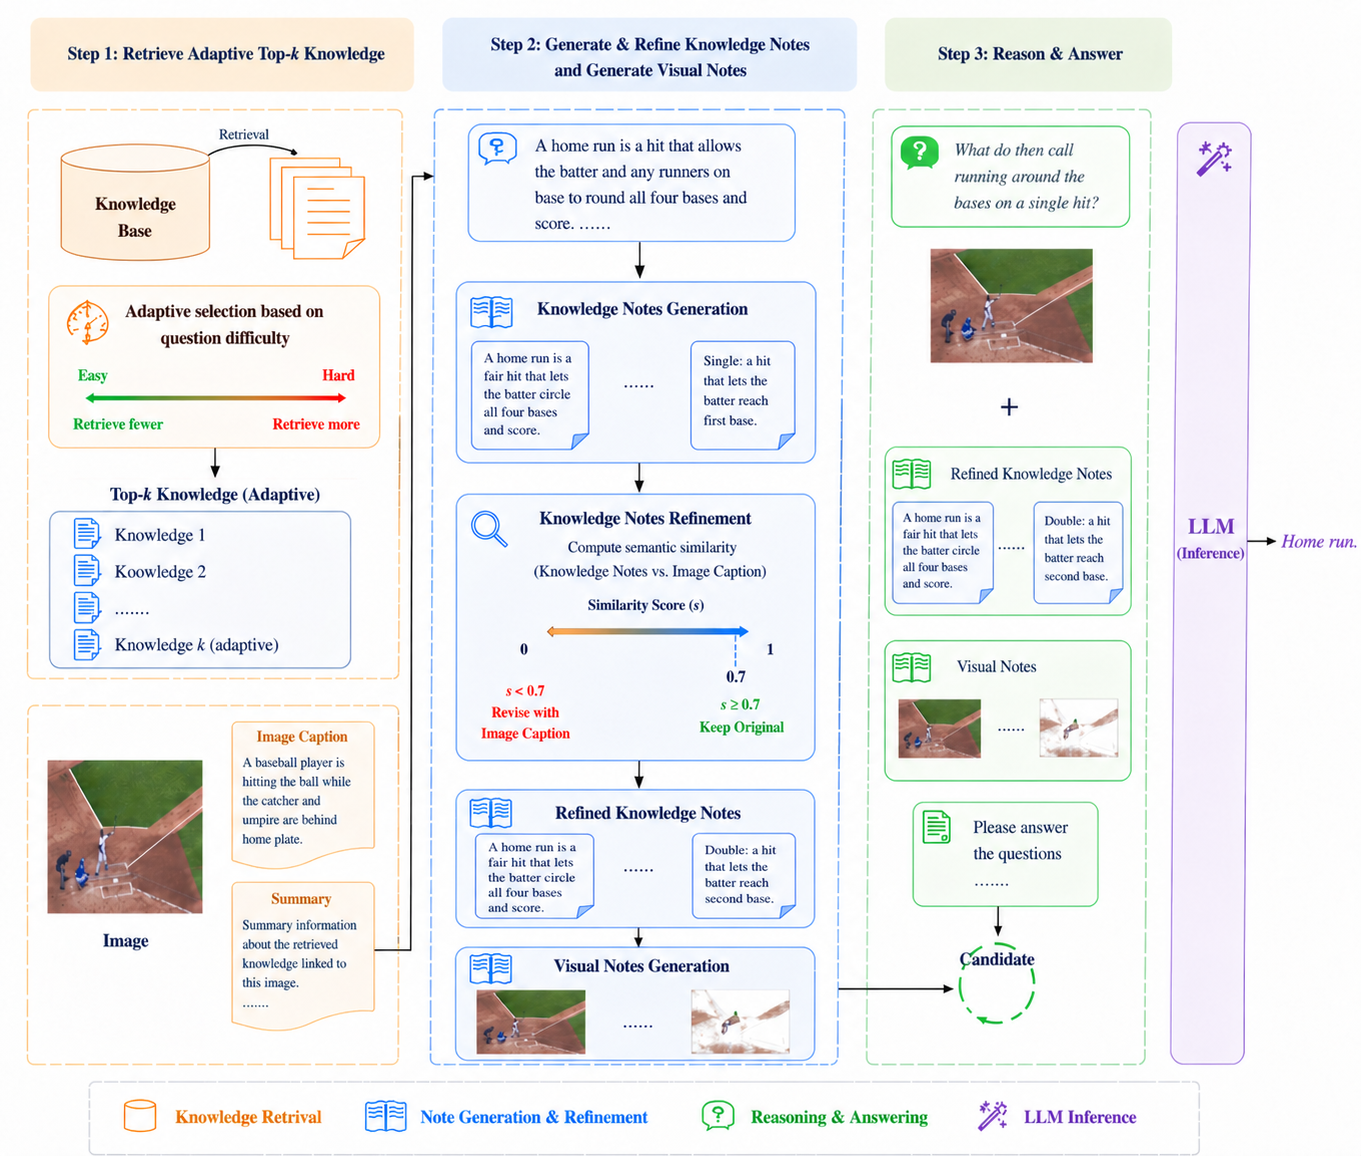
\includegraphics[width=0.8\textwidth]{DaCC-4.png}
  \caption{Overall framework of the proposed difficulty-adaptive and caption-consistent notes-guided reasoning method for KB-VQA.}
  \Description{Framework diagram of the proposed KB-VQA method, including adaptive retrieval, knowledge notes generation, caption-guided correction, visual notes generation, and final answer reasoning.}
  \label{fig:framework}
\end{figure*}

\subsection{Adaptive Top-k Knowledge Retrieval}

In KB-VQA, different questions have different levels of knowledge dependency. Some questions can be answered with simple commonsense or visual recognition, while others require more complex external knowledge. Therefore, using a fixed number of retrieved passages for all questions is suboptimal. Retrieving too few passages may lead to insufficient knowledge coverage, while retrieving too many passages may introduce noise and distract the MLLM during reasoning.

To overcome this limitation, we propose an adaptive top-$k$ knowledge retrieval strategy. The key idea is to estimate the difficulty of each image-question pair and dynamically select the number of retrieved knowledge passages.

Given an image $V$ and a question $q$, we first extract multimodal representations from both inputs. The question is encoded by a text encoder $F_L$, while the image is encoded by an image encoder $F_V$. To align visual features with textual features, we project the image representation into the shared semantic space:
\begin{equation}
Q = [F_L(q), F_M(F_V(V))],
\end{equation}
where $F_M$ is a projection module and $Q$ denotes the multimodal query representation.

For each candidate knowledge passage $d \in \mathcal{K}$, we encode it using the same text encoder:
\begin{equation}
D = F_L(d).
\end{equation}

The relevance score between the image-question pair and the knowledge passage is calculated by a late-interaction matching function:
\begin{equation}
r(\bar{q}, d) = \sum_{i=1}^{l_q} \max_{j=1}^{l_d} Q_i D_j^{T},
\end{equation}
where $\bar{q}$ denotes the multimodal query formed by the question and image, $l_q$ is the query length, and $l_d$ is the document length.

Instead of directly selecting a fixed number of top-ranked passages, we introduce a difficulty estimator to predict the required amount of external knowledge. The difficulty score is calculated from three complementary signals:
\begin{equation}
s_d = \alpha s_q + \beta s_r + \gamma s_m,
\end{equation}
where $s_q$ denotes the question complexity score, $s_r$ denotes the retrieval uncertainty score, and $s_m$ denotes the MLLM uncertainty score. The weights $\alpha$, $\beta$, and $\gamma$ control the contribution of different difficulty signals.

The question complexity score $s_q$ measures whether the question contains complex semantic structures or knowledge-dependent expressions. For example, questions involving abstract concepts, fine-grained categories, or causal reasoning are usually more difficult than simple object recognition questions.

The retrieval uncertainty score $s_r$ is calculated according to the distribution of retrieval scores. If the relevance scores of top-ranked passages are close to each other, the retriever is uncertain about which knowledge passage is most useful, indicating that more passages should be retrieved. We define:
\begin{equation}
s_r = 1 - (p_1 - p_2),
\end{equation}
where $p_1$ and $p_2$ are the normalized retrieval probabilities of the top-1 and top-2 passages. A smaller gap between $p_1$ and $p_2$ leads to a larger uncertainty score.

The MLLM uncertainty score $s_m$ measures how confident the MLLM is when answering the question without external knowledge. If the model produces unstable or inconsistent answers under multiple sampling attempts, the question is considered difficult and requires more external knowledge.

After obtaining the final difficulty score $s_d$, we compute the adaptive retrieval number:
\begin{equation}
k^{*} = \text{clip}\left(k_{\min} + \left\lfloor (k_{\max} - k_{\min}) s_d \right\rfloor, k_{\min}, k_{\max}\right),
\end{equation}
where $k_{\min}$ and $k_{\max}$ are the minimum and maximum numbers of retrieved knowledge passages. In this way, easy questions are assigned a smaller $k^{*}$, reducing redundant knowledge and computational cost, while difficult questions are assigned a larger $k^{*}$, improving knowledge coverage.

Finally, the retrieved knowledge set is obtained as
\begin{equation}
P_{k^{*}} = \text{Top-}k^{*}(\mathcal{K}, r(\bar{q}, d)).
\end{equation}
This adaptive retrieval strategy allows the model to retrieve knowledge according to the actual reasoning demand of each question, rather than using a fixed retrieval number for all samples.

\subsection{knowledge notes generation and correction}

After obtaining the adaptive retrieved knowledge passages $P_{k^{*}}$, we generate knowledge notes to summarize the most relevant information. Directly feeding raw retrieved knowledge into the MLLM may introduce noise, because retrieved passages often contain redundant, incomplete, or misleading information. Therefore, we use the MLLM to filter and reorganize the retrieved passages into concise and task-relevant knowledge notes.

Specifically, we provide the frozen MLLM with the image $V$, question $q$, and the retrieved knowledge set $P_{k^{*}}$. The MLLM is prompted to identify knowledge that is useful for answering the question and remove irrelevant content:
\begin{equation}
N_k^{0} = \text{MLLM}(V, q, P_{k^{*}}, c_k),
\end{equation}
where $N_k^{0}$ denotes the initial knowledge notes and $c_k$ is the knowledge notes generation prompt.

The prompt $c_k$ is designed to encourage the MLLM to perform three operations. First, it should judge whether each retrieved passage is related to the image and the question. Second, it should remove irrelevant or misleading information from the retrieved passages. Third, it should supplement necessary implicit knowledge if the retrieved passages are incomplete but related to the question.

A typical prompt can be formulated as follows: ``Given the image, question, and retrieved knowledge passages, summarize the knowledge that is useful for answering the question. Remove irrelevant or misleading information and keep the notes concise.''

Through this process, the initial knowledge notes integrate both explicit knowledge from the external knowledge base and implicit knowledge from the MLLM. Compared with raw retrieved knowledge, knowledge notes are more compact and more suitable for downstream reasoning.

However, the generated knowledge notes may still suffer from semantic inconsistency. If the retrieved knowledge is biased or only weakly related to the image, the MLLM may generate notes that are useful in a general textual sense but not grounded in the actual visual content. To address this problem, we further introduce a caption-guided semantic correction mechanism.

The core difference between our method and previous notes-guided reasoning frameworks lies in the bidirectional correction mechanism. Previous methods mainly use knowledge notes to guide visual attention, which can be regarded as a knowledge-to-vision process. However, if the knowledge notes themselves are not well aligned with the image, the generated visual notes may also be biased. To address this issue, we introduce an additional vision-to-knowledge correction process based on image captions.

Given the input image $V$, we first generate an image caption:
\begin{equation}
C = \text{Captioner}(V).
\end{equation}
The caption provides a compact semantic description of the image and serves as a visual semantic anchor. We then compute the semantic similarity between the image caption $C$ and the initial knowledge notes $N_k^{0}$.

Both $C$ and $N_k^{0}$ are encoded by a sentence-level text encoder $E(\cdot)$:
\begin{equation}
e_c = E(C), \quad e_n = E(N_k^{0}).
\end{equation}

The semantic similarity is calculated by cosine similarity:
\begin{equation}
\text{sim}(C, N_k^{0}) = \frac{e_c \cdot e_n}{\lvert e_c \rvert \lvert e_n \rvert}.
\end{equation}

We set a threshold $\tau$ to determine whether the knowledge notes are sufficiently aligned with the image caption. In our default setting, $\tau = 0.7$. If the similarity is higher than the threshold, the initial knowledge notes are regarded as visually consistent and are directly preserved:
\begin{equation}
N_k^{\text{corr}} = N_k^{0}, \quad \text{if } \text{sim}(C, N_k^{0}) \geq \tau.
\end{equation}

If the similarity is lower than the threshold, the initial knowledge notes may contain information that is inconsistent with the visual content. In this case, we use the image caption to revise the knowledge notes:
\begin{equation}
N_k^{\text{corr}} = \text{MLLM}(V, q, C, N_k^{0}, c_{\text{corr}}), \quad \text{if } \text{sim}(C, N_k^{0}) < \tau.
\end{equation}

Here, $c_{\text{corr}}$ is the correction prompt. It instructs the MLLM to remove knowledge that conflicts with the image caption and preserve knowledge that is useful for answering the question. A typical correction prompt is: ``Given the image, question, image caption, and initial knowledge notes, revise the knowledge notes. Remove information that is inconsistent with the image caption, keep useful knowledge for answering the question, and rewrite the notes concisely.''

This correction mechanism forms a bidirectional reasoning process. On the one hand, the corrected knowledge notes guide the generation of visual notes, which corresponds to knowledge-to-vision guidance. On the other hand, the image caption checks and corrects the knowledge notes, which corresponds to vision-to-knowledge correction. These two directions complement each other: the knowledge notes help the model focus on task-relevant visual regions, while the image caption ensures that the knowledge notes remain grounded in the actual image content.

\subsection{Visual Notes Generation}

Visual notes are generated to enhance the fine-grained visual perception of the MLLM. Although MLLMs have strong multimodal reasoning ability, they may still fail to attend to small but important regions in the image. For example, in KB-VQA, the answer may depend on a fine-grained object attribute, a small visual cue, or a specific region related to the retrieved knowledge.

To generate visual notes, we use the corrected knowledge notes $N_k^{\text{corr}}$ as textual guidance to identify image regions that are most relevant to the reasoning process. Given the input image $V$, we divide it into $M$ visual patches:
\begin{equation}
V_p = \{v_1, v_2, \ldots, v_M\}.
\end{equation}
Each patch $v_i$ is encoded into a visual feature vector. Meanwhile, the corrected knowledge notes $N_k^{\text{corr}}$ are encoded into textual feature representations. We then compute cross-modal attention between the visual patches and the textual tokens in the corrected knowledge notes.

Let $T = \{t_1, t_2, \ldots, t_L\}$ denote the token representations of the corrected knowledge notes, where $L$ is the number of textual tokens. The attention score between the $i$-th textual token and the $j$-th visual patch is calculated as
\begin{equation}
A_{i,j} = \text{softmax}\left(\frac{(t_i W_q)(v_j W_k)^T}{\sqrt{d}}\right),
\end{equation}
where $W_q$ and $W_k$ are learnable projection matrices and $d$ is the hidden dimension.

Based on the cross-modal attention scores, we generate a visual mask to select regions that are highly related to the corrected knowledge notes:
\begin{equation}
M_{i,j} =
\begin{cases}
1, & A_{i,j} > \lambda, \\
0, & \text{otherwise},
\end{cases}
\end{equation}
where $\lambda$ is the threshold for selecting important visual regions.

The final visual notes $N_v$ are obtained by applying the mask to the original image:
\begin{equation}
N_v = V \odot M,
\end{equation}
where $\odot$ denotes element-wise multiplication.

The generated visual notes preserve the regions that are most relevant to the corrected knowledge notes and suppress irrelevant background information. Since the visual notes are guided by semantically corrected knowledge notes, they are less likely to focus on regions caused by noisy or inconsistent knowledge. Therefore, the visual notes can better support the MLLM in fine-grained visual reasoning and reduce hallucination.

\subsection{Answer Reasoning}

Finally, the corrected knowledge notes $N_k^{\text{corr}}$, visual notes $N_v$, original image $V$, and question $q$ are combined as the final reasoning input:
\begin{equation}
X = \{V, q, N_k^{\text{corr}}, N_v\}.
\end{equation}

The answer is generated by the frozen MLLM:
\begin{equation}
\hat{y} = \text{MLLM}(X, c_a),
\end{equation}
where $c_a$ is the answer generation prompt. The prompt $c_a$ is designed to encourage the MLLM to integrate all available information and produce a concise answer. A typical answer generation prompt is: ``Given the image, question, knowledge notes, and visual notes, answer the question concisely based on the provided evidence.''

By adaptively controlling the amount of retrieved knowledge and correcting knowledge notes through visual semantic consistency, our method reduces knowledge noise, improves visual grounding, and enhances the reliability of MLLM reasoning for KB-VQA.

\section{Experiments}

\subsection{Datasets and Settings}

We evaluate the framework on two representative KB-VQA benchmarks, OK-VQA and A-OKVQA, which require the model to combine visual understanding with external knowledge. We follow the standard splits and report conventional VQA accuracy. The base reasoner is an MLLM in the BLIP-2 family, and retrieval is performed over a large external text corpus built from Wikipedia-style resources and web-accessible knowledge collections.

\subsection{Main Results}

Our method improves over strong retrieval-augmented baselines on both benchmarks. The gains are especially notable on questions that require functional, commonsense, or multi-step factual reasoning, suggesting that adaptive evidence selection and multimodal refinement are more effective than directly passing a fixed set of raw passages to the reasoner.

\subsection{Ablation Summary}

A compact ablation analysis shows that both core modules are necessary. Removing adaptive top-$k$ retrieval reduces answer accuracy because difficult questions no longer receive sufficient evidence coverage, while removing bidirectional refinement increases noise and weakens visual grounding. The full model performs best because it jointly controls retrieval breadth and evidence quality.

\section{Conclusion}

In this paper, we presented a framework for Knowledge-based VQA that optimizes the interaction between external knowledge and visual reasoning. By introducing an adaptive top-k retrieval strategy and a bidirectional refinement mechanism, we successfully minimize noise and maximize the relevance of retrieved facts. Our method sets a new state-of-the-art on the OK-VQA and A-OKVQA datasets, proving that intelligent knowledge management is as critical as reasoning capacity in multimodal tasks. Future work will explore the application of this refinement mechanism to real-time web-scale retrieval.

\bibliographystyle{ACM-Reference-Format}

\end{document}
